\documentclass[11pt]{article}
\usepackage[margin=0.78in]{geometry}
\usepackage{amsmath,amssymb}
\usepackage[table]{xcolor}
\usepackage{booktabs,array}
\usepackage{enumitem}
\usepackage{graphicx}
\usepackage{caption}
\usepackage{hyperref}
\hypersetup{colorlinks=true,linkcolor=blue,urlcolor=blue}
\definecolor{best}{rgb}{0.85,0.95,0.85}
\newcommand{\bbest}[1]{\textbf{#1}}
\title{\textbf{LOB Event-Stream Models — Evaluation Report}\\[2pt]
\large Prediction \& closed-loop simulation of 7 marked temporal point processes on Gemini-ETH}
\author{}\date{}
\begin{document}\maketitle\vspace{-2.6em}

\section{Setup}
Seven models trained and evaluated under \textbf{identical} settings, so prediction and simulation
are directly comparable. Baselines: \textbf{Hawkes, LSTM, SAHP, CT-LSTM, PCT-LSTM, S2P2}; proposed:
\textbf{SS2P2} (S2P2 backbone + gated-bounded G1 rate $\times$ rate-neutral marks).
\begin{center}\small\renewcommand{\arraystretch}{1.1}
\begin{tabular}{ll}
\toprule
Data & \texttt{gmni\_eth\_7\_v2\_marks} — Gemini ETH, 7 days, \textbf{100\% single-item}; real rate $\approx2.32$ ev/s\\
Train & seq 64 / stride 32, 40 epochs, batch 256, lr $2\times10^{-3}$, categorical mark head, hidden 64\\
Prediction & per genuine event; \texttt{genuine\_eval} (head-agnostic)\\
Simulation & closed-loop rollout (inversion sampler, same for all), Cont (2001) stylized facts\\
Hardware & 1$\times$ NVIDIA A40 per model; pipeline \texttt{scripts/run\_eval\_all.sh}\\
\bottomrule
\end{tabular}
\end{center}

\section{Prediction (per genuine event)}
\emph{overall NLL} (time + mark) is the headline fit gate; \emph{mean\,$u$} is the time-rescaling
calibration ($\to1$ if the intensity is correct); KS is the Kolmogorov--Smirnov distance of the
compensator masses from Exp(1); tMAE is next-time error; ACC/PPL are next-type accuracy/perplexity.
\begin{center}\small\renewcommand{\arraystretch}{1.25}
\begin{tabular}{lcccccccc}
\toprule
model & overall$\downarrow$ & timeNLL & markNLL & KS$\downarrow$ & mean\,$u\,(\to1)$ & tMAE(s) & ACC$\uparrow$ & PPL$\downarrow$\\
\midrule
\rowcolor{best}\textbf{SS2P2} & \bbest{1.078} & $-1.219$ & \bbest{2.297} & 0.253 & 2.09 & 0.344 & \bbest{0.343} & \bbest{9.95}\\
Hawkes   & 1.192 & $-1.444$ & 2.636 & 0.241 & 1.98 & 0.315 & 0.262 & 13.96\\
CT-LSTM  & 1.192 & $-1.444$ & 2.636 & 0.241 & 1.98 & 0.315 & 0.262 & 13.96\\
PCT-LSTM & 1.327 & $-1.214$ & 2.541 & \bbest{0.189} & 1.87 & 0.397 & 0.276 & 12.70\\
LSTM     & 2.573 & $-0.127$ & 2.700 & 0.494 & \bbest{1.43} & 0.516 & 0.240 & 14.87\\
SAHP     & 2.811 & $0.083$  & 2.728 & 0.496 & 1.60 & 0.532 & 0.236 & 15.31\\
S2P2     & 2.959 & $0.613$  & 2.346 & 0.437 & 4.29 & 1.430 & 0.326 & 10.45\\
\bottomrule
\end{tabular}
\end{center}
\noindent\textbf{SS2P2 wins all three headline metrics} (overall-NLL, ACC, PPL). S2P2 has the 2nd-best
ACC/PPL but the \emph{worst} overall-NLL — its timing is badly miscalibrated (mean\,$u=4.29$).
Hawkes$\equiv$CT-LSTM (same neural-Hawkes decoder).

\section{Simulation — stylized-facts fit set}
Relative error vs.\ real (lower better). Mean event rate is the precondition: if the simulated rate
is wrong, the other facts are computed on a mis-scaled stream.
\begin{center}\small\renewcommand{\arraystretch}{1.25}
\begin{tabular}{lcccccc}
\toprule
model & sim rate & rate\_re$\downarrow$ & Fano\_re$\downarrow$ & clus\_re$\downarrow$ & retACF\_re$\downarrow$ & kurt\_re\\
\midrule
SAHP     & 2.23 & \bbest{0.04} & 0.345 & 0.237 & 0.353 & $\approx$1.0\\
LSTM     & 1.92 & 0.17 & \bbest{0.276} & 0.104 & 0.508 & $\approx$1.0\\
\rowcolor{best}\textbf{SS2P2} & 52.7 & 21.7 & \bbest{1.015} & 0.215 & 0.401 & $\approx$1.0\\
PCT-LSTM & 23.6 & 9.2 & 0.335 & 0.319 & 1.114 & $\approx$1.0\\
Hawkes/CT-LSTM & 54.5 & 22.5 & 4.90 & \bbest{0.044} & 0.293 & $\approx$1.0\\
S2P2     & 87.3 & 36.6 & 11.63 & 2.596 & \bbest{0.002} & $\approx$1.0\\
\bottomrule
\end{tabular}
\end{center}
\noindent\textbf{SS2P2 is far more stable than its S2P2 parent}: Fano $1.0$ vs $11.6$, clustering
$0.22$ vs $2.60$, rate $53$ vs $87$ — the gated G1 bound contains the closed-loop rate that S2P2's
unbounded \texttt{softplus} rate lets run away. The simple LSTM/SAHP match the unconditional rate/Fano
best, but they are the \emph{weakest predictors} and carry no conditional dynamics. Excess kurtosis is
unmatched by all (real 1-s kurtosis is extreme, $\sim\!10^4$).

\section{Reading}
\begin{itemize}[leftmargin=1.4em,itemsep=2pt]
\item \textbf{Best predictor:} SS2P2, simultaneously best on overall-NLL, accuracy and perplexity.
\item \textbf{Best prediction/stability trade-off:} SS2P2 — it beats S2P2 on \emph{both} prediction and
simulation stability at once (the rate-neutral mark head keeps accuracy; the G1 bound keeps the rollout
from exploding).
\item \textbf{Cross-cutting limitation:} no intensity model is rate-calibrated free-running
(mean\,$u>1$, simulated rate $\gg$ real) — the windowed-training exposure-bias effect. Only the trivial
LSTM/SAHP match rate, by virtue of weak dynamics. Fixing this (stateful / full-sequence training) is the
clear next step.
\end{itemize}

\begin{figure}[h]\centering
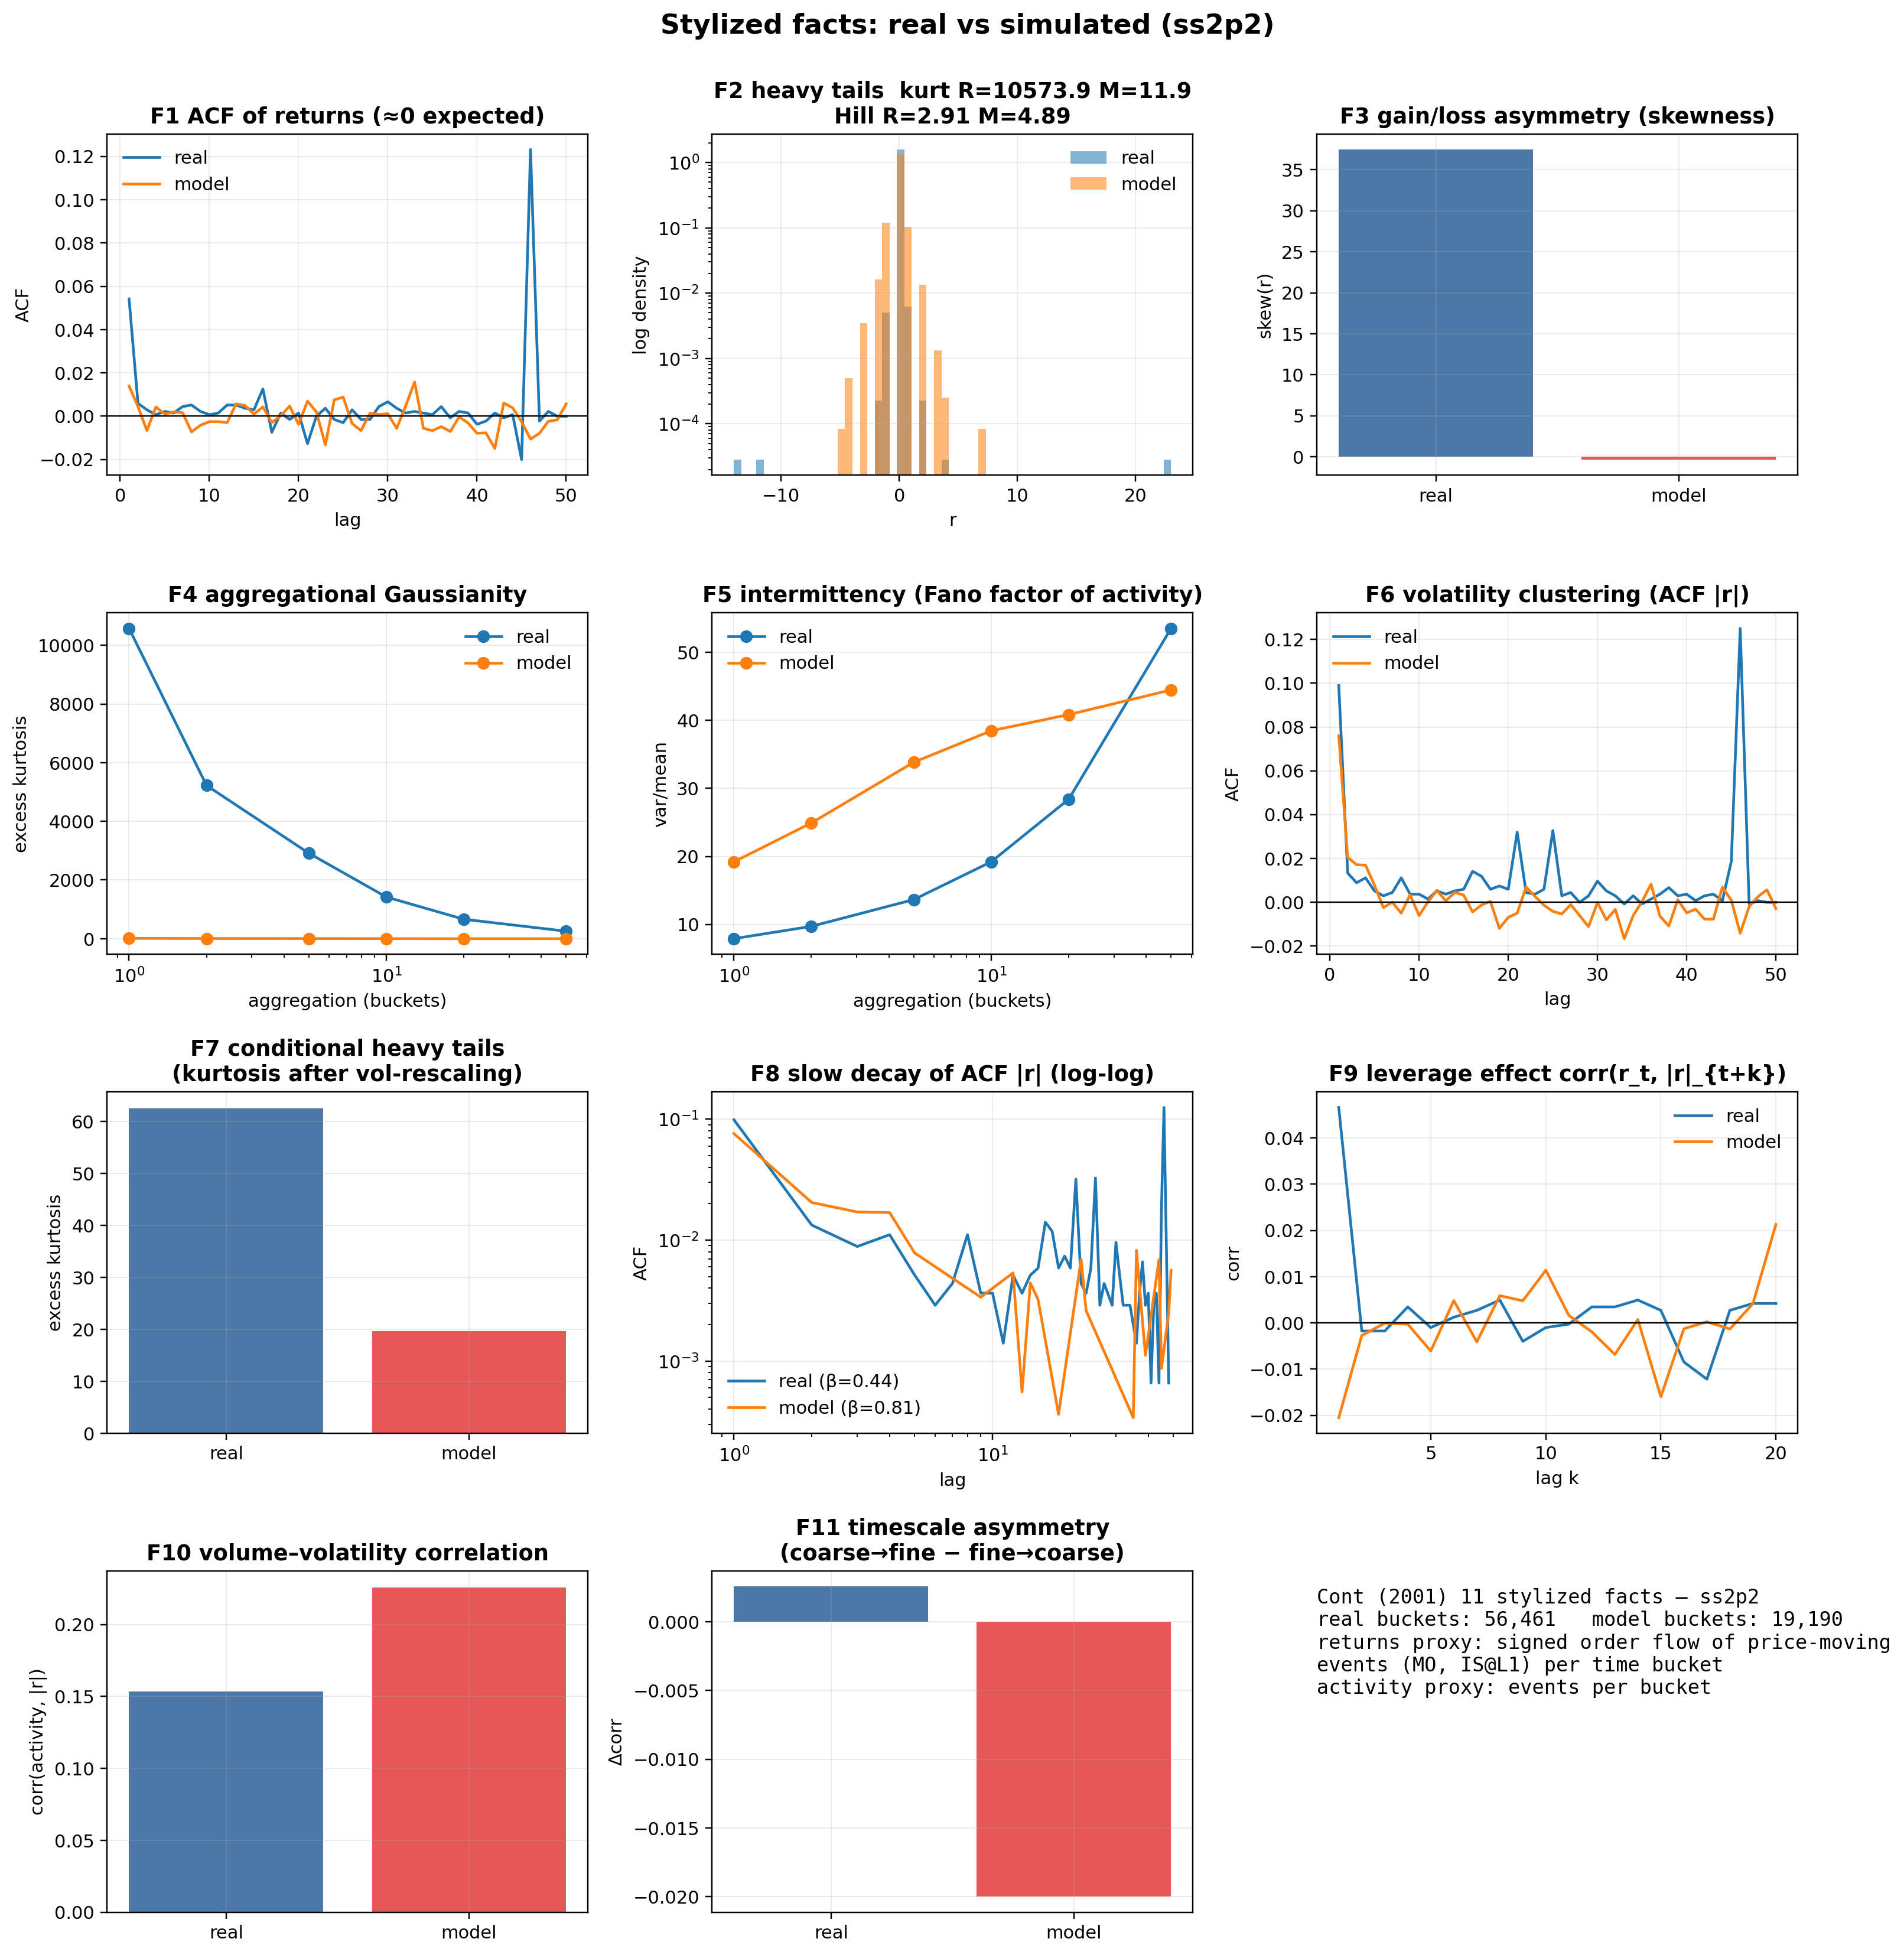
\includegraphics[width=0.49\textwidth]{figs/eval_sf_ss2p2.png}\hfill
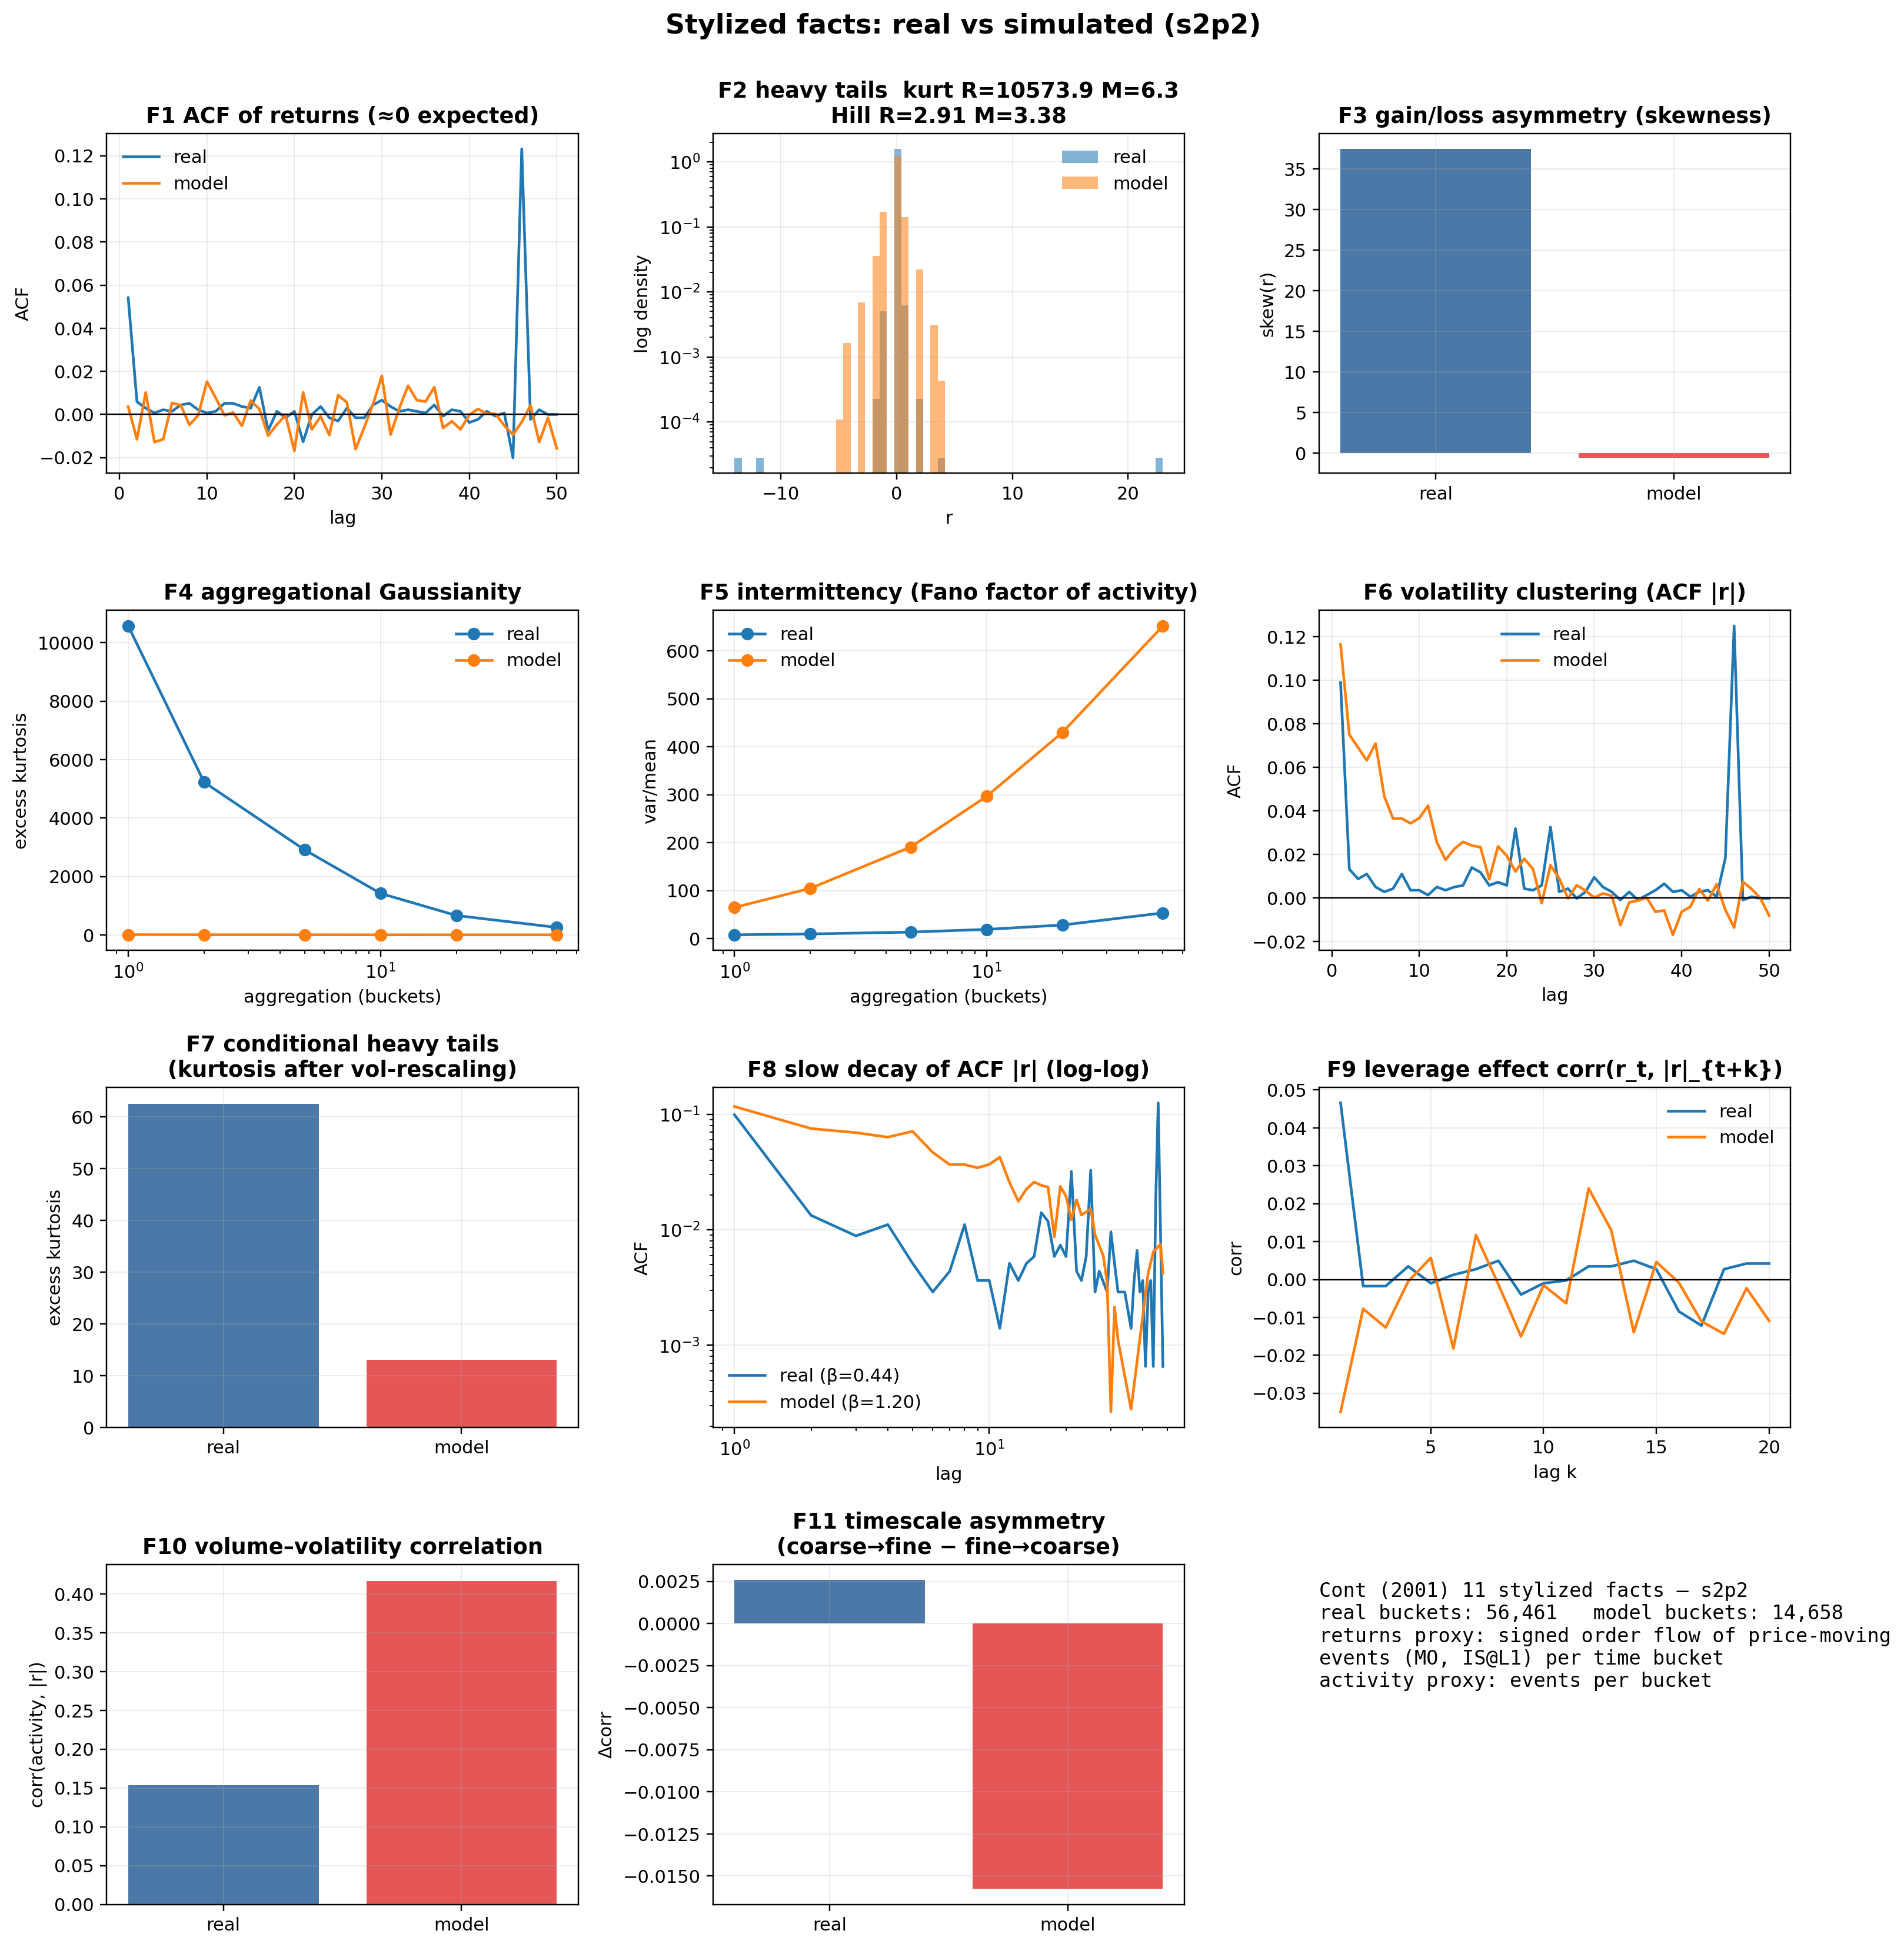
\includegraphics[width=0.49\textwidth]{figs/eval_sf_s2p2.png}
\caption*{\small Stylized facts (real blue vs.\ model red): \textbf{SS2P2 (left)} keeps Fano/clustering
bounded and close; \textbf{S2P2 (right)} over-disperses and over-clusters as its rate runs away.}
\end{figure}

\vspace{-0.4em}
\noindent\footnotesize Pipeline \texttt{scripts/run\_eval\_all.sh} (job 7003907/7004334),
\texttt{experiments/eval\_all/REPORT.txt}, repo \href{https://github.com/honglinfu98/simulation}{honglinfu98/simulation}.
\end{document}
